\documentclass[output=paper,colorlinks,citecolor=brown]{langscibook}
\ChapterDOI{10.5281/zenodo.15689135}
\author{Bettelou Los\affiliation{University of Edinburgh} and Stefano Coretta\affiliation{University of Edinburgh}}
\title{V2-relatives in Old English}
\abstract{The verb-placement asymmetry between main (verb-second, “V2”) and subclauses (\isi{verb-final}) found in Dutch and German is less pronounced in Old English (OE) \citep{Pintzuk1999}; the question is to what extent, as the distinction between main and subclauses cannot readily be determined on the basis of punctuation or other typographical conventions. It has long been noted that Old English shows constructions similar to the “V2-relatives” in modern Dutch and German \citep[188]{Mitchell1985}, while being much more difficult to identify. This paper proposes that the discourse functions of such clauses in Dutch and German might be used as a diagnostic for V2-relatives in OE, as these clauses tend to be used for “second mentions” of a major protagonist who has just been introduced. V2-relatives are less embedded than other relative clauses, and can be argued to represent a midway point in the grammaticalization of relatives, from a paratactic to a hypotactic structure. Key here is the difference between a demonstrative and the relative pronoun that developed from it.}

\IfFileExists{../localcommands.tex}{
  \addbibresource{../localbibliography.bib}
  \usepackage{langsci-optional}
\usepackage{langsci-gb4e}
\usepackage{langsci-lgr}

\usepackage{listings}
\lstset{basicstyle=\ttfamily,tabsize=2,breaklines=true}

%added by author
% \usepackage{tipa}
\usepackage{multirow}
\graphicspath{{figures/}}
\usepackage{langsci-branding}

  
\newcommand{\sent}{\enumsentence}
\newcommand{\sents}{\eenumsentence}
\let\citeasnoun\citet

\renewcommand{\lsCoverTitleFont}[1]{\sffamily\addfontfeatures{Scale=MatchUppercase}\fontsize{44pt}{16mm}\selectfont #1}
  
  %% hyphenation points for line breaks
%% Normally, automatic hyphenation in LaTeX is very good
%% If a word is mis-hyphenated, add it to this file
%%
%% add information to TeX file before \begin{document} with:
%% %% hyphenation points for line breaks
%% Normally, automatic hyphenation in LaTeX is very good
%% If a word is mis-hyphenated, add it to this file
%%
%% add information to TeX file before \begin{document} with:
%% %% hyphenation points for line breaks
%% Normally, automatic hyphenation in LaTeX is very good
%% If a word is mis-hyphenated, add it to this file
%%
%% add information to TeX file before \begin{document} with:
%% \include{localhyphenation}
\hyphenation{
affri-ca-te
affri-ca-tes
an-no-tated
com-ple-ments
com-po-si-tio-na-li-ty
non-com-po-si-tio-na-li-ty
Gon-zá-lez
out-side
Ri-chárd
se-man-tics
STREU-SLE
Tie-de-mann
}
\hyphenation{
affri-ca-te
affri-ca-tes
an-no-tated
com-ple-ments
com-po-si-tio-na-li-ty
non-com-po-si-tio-na-li-ty
Gon-zá-lez
out-side
Ri-chárd
se-man-tics
STREU-SLE
Tie-de-mann
}
\hyphenation{
affri-ca-te
affri-ca-tes
an-no-tated
com-ple-ments
com-po-si-tio-na-li-ty
non-com-po-si-tio-na-li-ty
Gon-zá-lez
out-side
Ri-chárd
se-man-tics
STREU-SLE
Tie-de-mann
}
  \boolfalse{bookcompile}
   \togglepaper[23]%%chapternumber
}{}

\begin{document}
\maketitle 


\section{Introduction} \label{sec:los:1}

In the modern West Germanic languages, movement of the finite verb to second position (“\isi{verb-second}” or “V2\is{verb-second}”) is a main clause phenomenon, and hence leads to a word order asymmetry between main (V2\is{verb-second}) and subclauses (\isi{verb-final}). Although the consensus is that \ili{Old English} is also a V2\is{verb-second}-language, albeit with some modifications (\citealt{vanKemenade1987}, see also \sectref{sec:los:2.4} below), the asymmetry between main and subclause is less pronounced \citep{Pintzuk1999}. Main and subclauses, and sentences in general, are not distinguished in the manuscripts by a consistent punctuation system, which adds to the challenges of determining the extent of the asymmetry. There is one type of clause in particular that has long been known to be analytically ambiguous (\citealt[86]{Allen1977}, \citealt[88]{Mitchell1985}), and may well be a contributing factor to the difficulty of establishing to what extent OE\il{Old English} exhibits the word order asymmetry found in the modern West Germanic languages:\footnote{The demonstrative form is in bold, and the finite verb is underlined; they will be marked like this throughout the paper; also note that the demonstrative, the source of the ambiguity, will be glossed as \textit{se}, and will be variously translated as a \isi{relative pronoun}, a demonstrative pronoun or a personal pronoun.}

\ea\label{ex:los:01}
\gll Maurus gemette ænne man eft \textbf{se} \underline{wæs} yfele getawod\\
Maurus met a man afterwards \textsc{se.nom.m} was evilly stricken \\
\glt ‘Maurus met a man afterwards who was evilly stricken.'\\ \hfill [ÆLS[Maur]:283.1661]
\z

\ea\label{ex:los:02}
\gll And Maurus ða gemette ær he to mynstre come ænne dumbne cnapan ⁊ \textbf{se} \underline{wæs} creopere eac\\
and Maurus then met before he to monastery came a dumb boy and \textsc{se.nom.m} was cripple too\\
\glt‘and Maurus then met before he came to the monastery a dumb boy and he was a cripple as well.' \hfill [ÆLS[Maur]:19.1507--8]
\z

For OE\il{Old English}, syntactic investigations have been able to rely on the York-Toronto-Helsinki Parsed Corpus of \ili{Old English} Prose (\isi{YCOE}, \citealt{TaylorTaylor2003}), a 1.5 million word corpus of \ili{Old English} prose based on the 1981 release of the Toronto \textit{Dictionary of Old English Corpus}, containing all the major \ili{Old English} prose \linebreak[4]works. Each word of the corpus is tagged for part of speech, and syntactically annotated by labelled bracketing in the Penn Treebank format, which has since become the industry standard for syntactic annotation. Data can be retrieved by CorpusSearch 2 (\citealt{Randall2005}–2007).

In \isi{YCOE}, \REF{ex:los:01} has been coded as a \isi{relative clause}, and hence as a subclause (IP-SUB), whereas \REF{ex:los:02} has been coded as a main clause (IP-MAT), in spite of their very similar structures including their main-clause-like word order with V2\is{verb-second}. It may well be the presence of the Tironian sign ‘⁊' for “and” in \REF{ex:los:02} that guided the annotator to an analysis of a sentence consisting of two main clauses rather than a main clause and an embedded clause, which is the analysis suggested by the coding of \REF{ex:los:01}. In the PDE translation in \citeauthor{Skeat1966}'s (\citeyear{Skeat1966} [1881–1900]) edition of \isi{Ælfric}'s \textit{Saints Lives} from which (\ref{ex:los:01}--\ref{ex:los:02}) have been taken, cases like \REF{ex:los:01} are routinely translated by relative clauses,\is{relative clause} and the \textit{se}{}-strategy is recognized as one of a range of relativizing strategies available in OE\il{Old English}, so, from that perspective, the interpretation of clauses like \REF{ex:los:01} as relatives is unproblematic. What poses a problem, however, is that relative clauses\is{relative clause} are not necessarily subordinate clauses – they may also be independent main clauses, and hence have main clause word order. Coding these as IP-SUB will boost the number of subordinate clauses in the data that have the same word order as main clauses, and hence obscure the word order asymmetry between main and subclauses in OE\il{Old English}. That OE\il{Old English} is an asymmetrical V2\is{verb-second} language is already clear from \posscitet{vanKemenade1987,vanKemenade1997} work; see also \citet[403--405]{Taylor2014}, and particularly \citet{MeklenborgSalvesen2017}, who conclude from their investigation of OE\il{Old English} \textit{þæt}{}-complement clauses that OE\il{Old English} does not allow embedded V2\is{verb-second}. This paper adds some further data to these insights as they pertain to relative clauses\is{relative clause}, and shows that the specific characteristics of V2\is{verb-second}-relatives echo those found in modern West Germanic, and lead to their specific \isi{discourse function} of marking a newly introduced protagonist.

This paper will look at all relative clauses\is{relative clause} in two OE\il{Old English} texts: \isi{Ælfric}'s \textit{Lives of Saints}\is{Ælfric's Lives of Saints} (\citet{Skeat1966} [1881–1900]) and the H manuscript (H ms, or ms H) of \textit{Gregory's Dialogues}\is{Gregory's Dialogues} (\cite{Hecht1965} [1900–1907]), and compare the use of \textit{se}{}-relatives with the other types of relative in terms of position of the verb, discourse functions\is{discourse function}, and antecedents. The paper is structured as follows: \sectref{sec:los:2} will present the types of relative clauses\is{relative clause} that have been identified for OE\il{Old English}: \textit{þe}{}-relatives, which are marked only by the invariant complementizer \textit{þe}, the “universal embedder”; \textit{se þe}{}-relatives, which are marked by the universal embedder as well as a demonstrative pronoun; and \textit{se}{}-relatives, which are marked only by the pronoun, and which are the focus of the investigation. \sectref{sec:los:3} discusses what has been said about V2\is{verb-second}-relatives in the modern West Germanic languages. \sectref{sec:los:4} and \sectref{sec:los:5} present the data and the methodology; as expected, it is the \textit{se}{}-relative that shows the highest frequencies of V2\is{verb-second}. What is new is that they serve a particular \isi{discourse function} in narrative in that they instantiate the \isi{second mention} of a newly-introduced protagonist. \sectref{sec:los:6} will place these findings in the wider context of the semantics of main and subclauses, and the development of \isi{hypotaxis}. \sectref{sec:los:7} concludes this paper.


\section{Typology of OE relatives} \label{sec:los:2}

\subsection{Introduction}\label{sec:los:2.1}
This section will provide a very brief overview of the main types of \isi{relative clause}s in OE\il{Old English}: \textit{þe}{}-relatives, \textit{se þe}{}-relatives and, finally, the \textit{se}{}-relatives, the type that our investigation into V2\is{verb-second}-relatives is most concerned with. For more detailed accounts, the reader is referred to the vast literature on the history of relative clauses\is{relative clause} in English that cannot be done justice here, see \citet{Allen1977}, \citet[$§§$2130ff]{Mitchell1985}, \citet[232]{Traugott1992}, \citet[659ff]{Fischer2000}, \citet{Suárez-Gómez2012}. 


\subsection{\textit{þe}-relatives}\label{sec:los:2.2}
Out of all types, the \textit{þe}{}-relative is the most frequent. In \isi{YCOE}, these are marked as having C occupied by \textit{þe} or \textit{ðe} while the Spec,CP position remains empty. \textit{Þe}{}-relatives are usually \isi{verb-final}, and restrictive. Unlike \textit{se}{}-relatives, they allow \isi{resumptive} pronouns\is{resumptive pronoun} and preposition stranding – evidence of a gap, and hence of movement/copying (\citealt{Allen1977}; \citealt{vanKemenade1987}). \textit{Þe} is a worn-down form of \textit{þæt} ‘that' which has become an invariant \textit{universal embedder} in OE\il{Old English}, marking not only relative clauses\is{relative clause} but also other clauses that we assume to be embedded (cf. Gothic \textit{ei}). The consensus in the literature is that \textit{þe}{}-relative clauses\is{relative clause} are embedded, and subordinate. Example \REF{ex:los:3} contains two \textit{þe}{}-relatives (\textit{þe} and \textit{ðe} in bold) as well as a \textit{se}{}-relative (\textit{ðone}); all three are coded as IP-SUB in \isi{YCOE}. \textit{Se}-relatives will be discussed in \sectref{sec:los:2.4}.

\ea
\label{ex:los:3}
\gll Sum æþel-boren þægn wæs philippus {gehaten ·} \textbf{ðone} \underline{asende} se casere Commodus \textbf{þe} on ðam {dagum ·} rixode fram rome byrig to ðære byrig \textbf{ðe} is gehaten alexandria\\
Some nobly-born thane was Philippus called \textsc{se.acc.m} sent the emperor Commodus \textsc{þe} on those days ruled from Rome city to the city \textsc{þe} is called Alexandria\\
\glt ‘A certain nobly-born thane was named Philip, who the emperor Commodus, who was in charge in those days, sent from the city of Rome to the city which is named Alexandria.' \hfill [ÆLS\_[Eugenia]:5.198]
\z

The second \textit{þe}-relative in \REF{ex:los:3} is restrictive, and postmodifies an NP (\textit{to ðære byrig} ‘to the city') that also contains a demonstrative form, the singular feminine \textit{ðære}, which is grammaticalizing\is{grammaticalization} into a \isi{definite article} in OE\il{Old English}; \textit{ðære} is used here to signal to the reader that they should be able to identify the referent, not because it has been mentioned in the earlier discourse (there is no earlier mention of a city which could be the antecedent) or because readers are expected to know it (unlike Rome), but because there is going to be a postmodifier (in the form of a \textit{þe}-relative) which will clarify what city is meant. \citet[172]{ArgüellesLos2022} identify this use of the \isi{definite article} as marking an important stage in the \isi{grammaticalization} process, namely, the stage at which definite articles\is{definite article} appear with a referent that is new in the discourse;\is{discourse-new} the use of the \isi{definite article} is “licensed” by a postmodifier that “activates the general knowledge necessary to locate the referents in a contextual set” \citep[74]{Wagener2017}. \citet{Breban2012} refers to them as “\isi{definite first mentions}”. Typically, such a use of the \isi{definite article} signifying identifiability is no longer compatible with a demonstrative reading. 

The first instance of the \textit{þe}{}-relative, however, is not restrictive – it postmodifies a named referent, as does the \textit{se}{}-relative with \textit{ðone}. The reason for this will be explored in \sectref{sec:los:3.4}.


\subsection{\textit{Se þe}-relatives} \label{sec:los:2.3}
\textit{Se þe}-relatives consist of a form of the distal \isi{demonstrative} \textit{se} as well as the embedder \textit{þe}. The distal \isi{demonstrative} doubles as the \isi{definite article} in OE\il{Old English}. Its paradigm is given in \tabref{tab:los:1}:

\begin{table}
\begin{tabularx}{\textwidth}{XXXXX} 
\lsptoprule
& \multicolumn{3}{c}{{singular}} & \multicolumn{1}{c}{plural}\\
\cmidrule(lr){2-4}\cmidrule(lr){5-5}
& {masculine} & {feminine} & {neuter} & {all genders}\\
\midrule
{nom} & {se} & {seo} & {þæt} & {þa}\\
{gen} & {þæs} & {þære} & {þæs} & {þara}\\
{dat} & {þæm} & {þære} & {þæm} & {þæm}\\
{acc} & {þone} & {þa} & {þæt} & {þa}\\
{instr} & \multicolumn{3}{c}{{þy, þon}} & \\
\lspbottomrule
\end{tabularx}
\caption{The paradigm of the distal demonstrative in OE}
\label{tab:los:1}
\end{table}

\textit{Se þe}-relatives have an inherent degree of ambiguity, as they may represent two or perhaps three separate types: (i) a \textit{þe}{}-relative that has a \isi{demonstrative} antecedent as an appositive NP with a restrictive \isi{relative clause}, comparable to PDE “i.e.” (\textit{hiera mægas him mid wæron} \textbf{\textit{þa} \textbf{þe}} \textit{him from noldon} ‘their kinsmen were with him, i.e. those who did not want to leave him' in [ChronA 755.1–29]); (ii) a \textit{þe}{}-relative whose \isi{demonstrative} antecedent has a syntactic function in the higher clause, comparable to the generic “free relative” use of PDE \textit{he that lives in a glass house should not throw stones} (\citealt{Allen1977}; see also \citealt{Allen2020} for more detail and analysis of this type); (iii) there is also the possibility that \textit{se} \textit{þe} is a “compound” relativizer. 

In \isi{YCOE}, types (i) and (ii) differ from each other in that type (ii) has an empty Spec,CP position, as the \isi{demonstrative} is best analyzed as a constituent of the higher clause, outside the \isi{relative clause}. We have followed \isi{YCOE} coding in our searches, which means that type (ii) will have been included under the \textit{þe}{}-relative. 

The \textit{se} \textit{þe}-relative has been described as “mostly restrictive” \citep{Mitchell1959}. \textit{Se} \textit{þe}-relatives are not found with preposition stranding, and this is the only type that exhibits “\isi{case attraction}”, a fairly rare phenomenon in the case of type (i), in which the \isi{demonstrative} appears with the case it would have if it was a constituent of the higher clause (\citealt[150]{vanKemenade1987}; \citealt{Allen2020}); this might be a kind of appositional use, see \textit{him} in the translation:

\ea\label{ex:los:4}
\gll ge seceað þone hælynd \textbf{þone} þe on rode ahangen wæs\\
you seek the.\textsc{acc} savior \textsc{se}.\textsc{acc.m} \textsc{þe} on cross hanged was\\
\glt ‘You seek the Savior, him, who was hanged on the cross.'\\ \hfill [cowsgosp,Mt\_[WSCp]:28.5.2139]; \citep[87]{Allen1977}
\z

\subsection{\textit{Se}-relatives} \label{sec:los:2.4}
\textit{Se}-relatives are the type that is the focus of this investigation. An example is \REF{ex:los:5}:

\ea\label{ex:los:5}
\gll Se feorða godspellere is Iohannes Cristes moddrian sunu, \textbf{se} \underline{wæs} Criste swa leof þæt he hlynode uppan his breoste.\\
the fourth gospelwriter is John Christ.\textsc{gen} aunt.\textsc{gen} son
\textsc{se.nom.m} was Christ.\textsc{dat} so dear that he leaned upon his breast \\
\glt ‘The fourth gospelwriter is John, Christ's aunt's son, who was so dear to Christ that he leaned upon his breast.' \hfill [ÆLS\_[Mark]:159.3304]
\z

\textit{Se}-relatives often have V2\is{verb-second} word order (\citealt{Allen1977}; \citealt[149]{vanKemenade1987}). They do not show \isi{case attraction}, and do not occur with resumptives\is{resumptive} or preposition stranding, that is, without a clear structural gap \citep{Wende1915, Allen1977}. \textit{Se}-relatives in OE\il{Old English} are, as a rule, non-restrictive (\citealt[131--132, 138]{LosvanKemenade2018}; \citealt{Roma2007}: 266), which are known to be less embedded than restrictive relatives: They do not define their antecedent but add extra information, and are less integrated\is{integration} into the structure of the higher clause from a syntactic, prosodic, and informational point of view \citep[1034--1035]{HuddlestonPullum2002}. Non-restrictive relative clauses\is{relative clause} in PDE are well-known to exhibit main clause behavior, such as verb phrase preposing, negative constituent preposing and \isi{topicalization} \citep{Emonds1970, HooperHooper1973, Green1976, deVries2012, Heycock2017}. In terms of \isi{discourse function}, they are often used for expressing the next event in a plotline as in \REF{ex:los:6} (foregrounding) but also for explanations, reasons and causes (backgrounding), as in \REF{ex:los:7}:

\ea\label{ex:los:6}
{\itshape She gave the letter to the clerk, who copied it.} \hfill \citep[699]{Depraetere1996}
\z

\ea\label{ex:los:7}
{\itshape If Peter called the dean, who hates me, I would be in trouble.}\\ \hfill \citep[142]{JasinskajaPoschmann2020}
\z

Another interesting use of relative clauses\is{relative clause} in Dutch is noted by \citet[183]{deVries2012} (\isi{relative clause} in bold):

 \ea\label{ex:los:8}
\gll Joop, \textbf{die} \textbf{nu} \textbf{zijn} \textbf{kamer} \textbf{gaat} \textbf{opruimen!}, komt straks buiten spelen.\\
Joop who now his room goes clean comes later outside play\\
\glt ‘Joop, who is now going to clean his room!, will come play outside later.'
\z

A sentence like \REF{ex:los:8} might be uttered by Joop's mother to a friend of Joop's who has presented himself at the door, importantly, within earshot of Joop; the non-restrictive \isi{relative clause} is, in fact, an order to Joop.

The most natural way to translate \textit{se}{}-relatives into PDE is with a \isi{relative clause}, particularly, if they have human antecedents, as in \REF{ex:los:5}. Although singular animate antecedents can be relativized by \textit{who} or \textit{that}, they no longer allow a translation by an independent \isi{demonstrative}, unless they are in the plural, witness the contrast between \REF{ex:los:9a} and \REF{ex:los:9b} below. Example \REF{ex:los:9c} shows “a contrast in animacy, \textit{he} referring to a person or animal, \textit{that} to an inanimate” \citep[1504--1505]{HuddlestonPullum2002}. Compare also the anaphoric uses in \xxref{ex:los:9d}{ex:los:9e}.


 \ea\label{ex:los:9}
\ea \label{ex:los:9a}
{\itshape \textbf{Those} who obtain a score of 90\% will win a prize.}
\ex\label{ex:los:9b}{
\itshape *\textbf{That} who obtains the highest score will win a prize.}
\ex \label{ex:los:9c}
{\itshape \textbf{He}/*\textbf{That} saved my life.}
\ex \label{ex:los:9d}
{\itshape The population of Victoria far exceeds \textbf{that} of Queensland.}
\ex \label{ex:los:9e}{
\itshape *The premier of Victoria will be meeting with \textbf{that} of Queensland.}\\ \hfill \citep[1504, their (3) i--v]{HuddlestonPullum2002} 
\z
\z

In Dutch and \ili{German}, main clauses headed by \isi{demonstrative} pronouns coerce \isi{topic shift} \citep{Comrie1997}: The implication of using a \isi{demonstrative} rather than a personal pronoun coerces interpreting the referent as a newly introduced one rather than as a \isi{continuing topic}. This is no longer the case in PDE, so that the referent of \textit{she} underlined in \REF{ex:los:10} is ambiguous – this is what makes the exchange interesting: 

\ea\label{ex:los:10}
Columbo: {\itshape No, my wife is not here. She had to go to Chicago to look after her mother. \underline{She} had a fall and broke her hip.}\\ Woman at party: {\itshape Oh, your wife broke her hip? How terrible.}\\ Columbo: {\itshape No, her mother.} \\
\hfill (Columbo, series 10.1, episode \textit{No time to die}; \\ \hfill \citep[134]{LosvanKemenade2018}
\z

The natural choice to disambiguate the two possible referents in Dutch and \ili{German} would be the personal pronoun for the continued topic (the wife) and the \isi{demonstrative} for the new\is{discourse-new} topic (the mother). In PDE, a \isi{relative clause} would have disambiguated the referent; “who had a fall and broke her hip” could only have referred to the mother. This suggests that (non-restrictive) relative clauses\is{relative clause} may have stepped in as a compensatory strategy once the topic shifting\is{topic shift} function of demonstratives\is{demonstrative} was lost; it also explains why a main clause headed by a “standalone” \isi{demonstrative} referring to a singular human antecedent is much more likely to be annotated as a \isi{relative clause} than as a main clause by annotators who, as in the case of \isi{YCOE}, tended to be native speakers of English. 

This loss in functionality of the singular \isi{demonstrative} is already evident in Early \ili{Middle English}, where one finds innovative periphrases – which did not catch on – \textit{he this, she this} (\citealt{Mustanoja1960}: 137; \citealt{Miura2016}) as translations for topic-shifting Latin \textit{iste}, indicating a need to restore the earlier functionality. The account provided in \citet{Allen2022} shows that \textit{se}-relatives – reduced to invariant \textit{þe} after the loss of the paradigm of \tabref{tab:los:1} – are no longer found after 1150 with antecedents in the previous discourse, only with generic referents in free relatives, corresponding to Present-Day English \textit{he who}; the loss of \isi{gender} is tentatively identified as being implicated, supporting a suggestion made in \citet{LosvanKemenade2018}, who point to the fact that the contrast in acceptability between singular and plural demonstratives\is{demonstrative} in PDE as in \REF{ex:los:9a} versus \REF{ex:los:9b} makes sense in the context of the OE\il{Old English} \isi{demonstrative} paradigm, which was gendered\is{gender} in the singular but not in the plural.

Cases like \REF{ex:los:5}, and the \textit{ðone}{}-clause in \REF{ex:los:3}, ambiguous between main clause and subclause, are the focus of the remainder of this paper. This ambiguity extends to standalone demonstratives\is{demonstrative} as complements of a preposition in a clause-initial PP, as in \REF{ex:los:11}:

\ea\label{ex:los:11}
\gll His wif wæs gecyged claudia be \textbf{þære} he \underline{\smash{gestrynde}} twægen {suna ·} {auitum ·} ⁊ {særgium ·} ⁊ ane dohtor eugenian þe we embe spræcaþ.\\
his wife was called Claudia by \textsc{se.dat.f} he had two sons Avitus and Sergius and one daughter Eugenia \textsc{þe} we about talked\\
\glt ‘His wife was called Claudia, by whom he had two sons, Avitus and Sergius, and one daughter Eugenia who we mentioned earlier.'\\ \hfill [ÆLS\_[Eugenia]:15.202]
\z

The fact that they do not allow preposition stranding, and thus always show “pied piping” as in \REF{ex:los:11}, has been argued to be evidence that \textit{se}{}-relatives involve movement or copying \citep[91]{Allen1977}. Note that the absence of stranding could equally well serve as evidence of main clause “Topicalization”\is{topicalization} (movement to the pre-field); PP-initial adjuncts linking to previous discourse are much more frequent in OE\il{Old English} than in later periods, particularly PPs that contain standalone demonstratives\is{demonstrative} as in \REF{ex:los:11}; see \citet{los2023decline} for the decline of such “local anchors” in the history of English. PDE favors subjects as the default expression of given information, so that a translation like \textit{by/with her he had two sons} is less felicitous in PDE than a \isi{relative clause} \textit{by/with whom he had two sons}. This is why such PPs, too, are much more likely to be annotated as relative clauses\is{relative clause} than as PP-initial main clauses. 

Note that the surface V3\is{verb-third}-order of \REF{ex:los:11} is part of the manner in which “V2\is{verb-second}” plays out in OE\il{Old English}: The finite verb will move to C in “\isi{focus}” contexts (interrogatives, negative initial constituents as well as the “narrative operator” \textit{þa} ‘then' as the first element). It will move to a lower head, however, if some other initial phrase, such as a PP, is occupying the prefield, which leads to surface V3\is{verb-third} if the subject is a pronoun, as in \REF{ex:los:11} \citep{vanKemenade1987}. This means that the sequence \textit{be þære he gestrynde} is a possible main clause order.

In \isi{YCOE}, \textit{se}{}-relative clauses\is{relative clause} receive a syntactic annotation in which the \isi{demonstrative} is in Spec,CP and C is empty (marked by “0”); as a relative, the clause-label indicates a subclause (IP-SUB). As an example, \REF{ex:los:12} shows the annotation of the \textit{ðone}{}-clause of \REF{ex:los:3}; \REF{ex:los:5} and \REF{ex:los:11} are annotated along similar lines.


 \ea\label{ex:los:12}
 (CP-REL-1 (WNP-ACC-4 (D\^{}A +done))\\
 ~~~~~~~~~~~~~~~~~~~~(C 0) \\
 ~~~~~~~~~~~~~~~~~~~~(IP-SUB (NP-ACC *T*-4)\\
 ~~~~~~~~~~~~~~~~~~~~~~~~~~~~~~~(VBD asende)\\
 ~~~~~~~~~~~~~~~~~~~~~~~~~~~~~~~(NP-NOM (D\^{}N se) (N\^{}N casere)\\
\z

An example of a standalone \isi{demonstrative} coded as heading a main clause is \REF{ex:los:13}, with the \isi{demonstrative} as a complement of a preposition:

 \ea\label{ex:los:13}
 \gll \& þa sealde he heom mid his agenre handa ane trywene \underline{\smash{flascan}} wines fulle, to þon þæt hi mihton heom \textbf{þa} on heora færelde to underngeweorce habban. Of \textbf{þære} hi druncon, oð þæt hi to rauennam becomon\\
and then gave he them with his own hands a wooden bottle of-wine full to that that they might for-themselves \textsc{se-acc.sg.F} in their journey for breakfast have from \textsc{se-dat.sg.F} they drank, until that they to Ravenna came\\
\glt ‘and then, with his own hands, he gave them a wooden bottle full of wine, so that they might have that for breakfast during their journey. They drank from it, until they arrived in Ravenna.' (i.e. it lasted them all the way to Ravenna) \hfill [GD\_1\_[C]:9.66.12.742--743]
\z

In \REF{ex:los:13}, a referent (a feminine noun meaning ‘bottle', underlined) is introduced and then referred back to by two instances of \textit{se} (in bold). The second instance, \textit{of þære}, receives the following syntactic annotation in \isi{YCOE}, with the clause-label indicating a main clause (IP-MAT):

 \ea\label{ex:los:14}
(IP-MAT (PP (P Of)\\
~~~~~~~~~~~~~~~(NP-DAT (D\^{}D +t+are)))\\
~~~~~~~~~~(NP-NOM (PRO\^{}N hi))\\
~~~~~~~~~~(VBDI druncon)\\
\z

What makes an analysis like \REF{ex:los:14} more likely for an example like \REF{ex:los:13} is the distance between the antecedent and the \isi{demonstrative}. Faced with a similar dilemma – \isi{demonstrative}-headed main clause or embedded relative? – in her \ili{Old High German} data, \citet{Schlachter2012} also uses distance between antecedent and \isi{demonstrative} to support a main clause analysis of analytically ambiguous \isi{demonstrative}-headed V2\is{verb-second} constructions.

The question is whether \REF{ex:los:3} (the ðone-clause), \REF{ex:los:5} and \REF{ex:los:11} should receive a syntactic annotation along the lines of \REF{ex:los:14}, with the \isi{demonstrative} (whether as part of a PP or as a subject or object) heading an independent main clause, rather than \REF{ex:los:12}, with the \isi{demonstrative} heading a subclause. \\


\section{V2-relatives in Dutch and German}\label{sec:los:3}

\subsection{Introduction}\label{sec:los:3.1}
The dilemma posed by \textit{se}-headed structures in OE\il{Old English} is presented in the literature as the choice of a main clause headed by a standalone \isi{demonstrative} versus an embedded \isi{relative clause}. The emphasis of the literature on V2\is{verb-second}-relatives in Dutch and \ili{German}, however, is not so much on the status of main versus \isi{relative clause} but on the difference between embedded and less embedded relative clauses\is{relative clause}. The analysis of main clauses headed by demonstratives\is{demonstrative} as separate sentences never seems to be in doubt, presumably given the clear markings of sentences in written texts by means of punctuation, and their intonational phrasing in speech. The discussions in \citet{Gärtner2001} and \citet{Zwart2003} among others focus on V2\is{verb-second}-clauses that are part of a sentence that includes a previous clause where the referent, typically, is newly-introduced, of the type of \xxref{ex:los:15b}{ex:los:15c}. The contrast, then, is between \REF{ex:los:15b} and the embedded, \isi{verb-final} \isi{relative clause} as in \REF{ex:los:15c}. 

 \ea\label{ex:los:15}
 \ea \label{ex:los:15a}
 \glll iemand \underline{had} twee zonen.\\
 someone had two sons\\
[main clause with V2]\\
 
 \ex \label{ex:los:15b}
 \glll Er was iemand \textbf{die} \underline{had} twee zonen. \\
there was someone that had two sons\\
[main clause + V2-relative]\\

 \ex \label{ex:los:15c}
\glll Er was iemand \textbf{die} twee zonen \underline{had}.\\
there was someone that two sons had\\
[main clause + embedded relative] \\
\glt ‘There was someone who had two sons.'
\z
\z

Both \citet{Gärtner2001} and \citet{DenDikken2003} discuss a third structure as in \REF{ex:los:16}, on the basis of an observation made by \citet[6]{Zwart2003} about responses to a 19th-century dialect questionnaire. This questionnaire presented the sentence in \REF{ex:los:15a} as the start of a story, its function being to introduce the father. The respondents subsequently gave \REF{ex:los:15b}, the V2\is{verb-second}-relative, but also, unexpectedly, \REF{ex:los:16}:

\ea \label{ex:los:16}
\glll Er was iemand en \textbf{die} \underline{had} twee zonen.\\
 there was someone and that had two sons\\
[main clause + main clause ]\\
\glt ‘There was someone and he had two sons.' 
\z

Example \REF{ex:los:16} contains two main clauses, the second headed by a standalone \isi{demonstrative}. These were apparently felt, by the repondents, to be equivalent, an indication that they both serve the same function. \citet[109]{Gärtner2001}, discussing a similar set of sentences (\textit{Es gibt Philosophen (und) die stammen aus Griechenland} ‘there are philosophers who come from Greece') notes that the main difference between the version with and without \textit{und} ‘and' is one of informational units – a \isi{relative clause}, whether V2\is{verb-second} or embedded, will form an informational unit, as also defined by their intonation/prosody (a rising tone before the \isi{relative clause}). In the version with \textit{und}, a “falling tone, drop, pause, or similar features” (p. 109) would be expected. This does not sufficiently explain the Dutch case of \REF{ex:los:16}, however, where the first main clause is just as uninformative as in \REF{ex:los:15}, and would not have a falling tone after \textit{iemand}. 

The different emphases in the various discussions can be visualized by the Venn diagram in \figref{fig:los:1}.

\begin{figure}
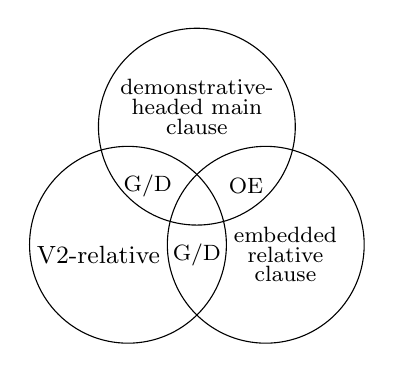
\begin{tikzpicture}[scale = 0.5] 
\draw  (0, 0) circle (2.5cm);
\draw  (3.5, 0) circle (2.5cm);
\draw  (1.75, 3) circle (2.5cm);

\node [font=\footnotesize] at (1.75, 4) {demonstrative-};
\node [font=\footnotesize] at (1.75, 3.5) {headed main};
\node [font=\footnotesize] at (1.75, 3) {clause};

\node [font=\small] at (-0.75, -0.25) {V2-relative};

\node [font=\footnotesize] at (4, 0.25) {embedded};
\node [font=\footnotesize] at (4, -0.25) {relative};
\node [font=\footnotesize] at (4, -0.75) {clause};

\node [font=\footnotesize] at (1.75,-0.25) {G/D};
\node [font=\footnotesize] at (0.5, 1.5) {G/D};
\node [font=\footnotesize] at (3, 1.5) {OE};
\end{tikzpicture}

 \caption{Focus of relevant investigations in the literature on OE and on \ili{German} (G) and Dutch (D)}
 \label{fig:los:1}
\end{figure}
 
The existence of the V2\is{verb-second}-relative as a less embedded \isi{relative clause} has not been mooted in the literature on OE\il{Old English} – the dilemma is, as far as we are aware, always presented as being between a \isi{relative clause} (assumed to be embedded by definition) and a main clause with a standalone, independent \isi{demonstrative}. We will see in the following sections that the tests put forward in the literature about Dutch and \ili{German} V2\is{verb-second}-relatives to untangle the three possibilities, that is, \REF{ex:los:15b}--\REF{ex:los:15c} and \REF{ex:los:16}, will be too fine-grained for OE\il{Old English}; but we will be able to say something about the embedded option versus the rest, at least in some OE\il{Old English} texts, and hence identify verb position as a fairly clear marker for less embedded relative clauses\is{relative clause}.


\subsection{Embedded relatives versus V2-relatives}\label{sec:los:3.2}
Various syntactic tests demonstrate that V2\is{verb-second}-relatives behave like main clauses, unlike more embedded relatives. Some tests require manipulation of the data and native speaker judgements about the results that are not available to investigators of a dead language, particularly, if these judgements “are sometimes subtle” \citep[104]{Gärtner2001}, and marked by “??” even by native speakers. The item that stands out as a potential feature to check in the OE\il{Old English} instances is the fact that the V2\is{verb-second}-relative needs to be clause-final (p. 100) – an indication, perhaps, like the main-clause characteristics found in the \ili{German} examples, that the V2\is{verb-second}-relative started out as a paratactic\is{parataxis} construction. 

Note that \citeauthor{Gärtner2001}'s (\citeyear{Gärtner2001}) paper provides a single PDE translation for his examples comparing V2\is{verb-second}-relatives with their more embedded counterparts, like \REF{ex:los:17a} and \REF{ex:los:17b}, as their meanings do not differ; Gärtner's notation (/) denotes that the V2\is{verb-second}-relative in \REF{ex:los:17a} is intonationally integrated\is{integration} into the previous clause, just like its more embedded \isi{relative clause} counterpart in \REF{ex:los:17b}; it forms a single informational unit with the matrix clause, just like an embedded relative (p. 109). V2\is{verb-second}-relatives like \REF{ex:los:17a} are, in fact, presented as variants that are felicitous only when certain conditions are met, unlike the embedded versions – in a V2\is{verb-second}-relative, the antecedent (\textit{eine Seite} in \REF{ex:los:17}) must be presentational\is{presentational constructions}, specific and indefinite:


 \ea\label{ex:los:17}
  \ea \label{ex:los:17a}
{\itshape Das Blatt hat eine Seite, (/) \textbf{die} \underline{ist} ganz schwarz.}
\ex \label{ex:los:17b}
{\itshape Das Blatt hat eine Seite, (/) \textbf{die} ganz schwarz \underline{ist}.}
\glt ‘The sheet has a side that is completely black.' \hfill \citep[98]{Gärtner2001}
\z
\z

The specificity-requirement is best illustrated by an example from \citet{ConiglioHinterhölzl2020}: 

\ea\label{ex:los:18}
\ea \label{ex:los:18a}
{\itshape Hans sucht eine Frau, \textbf{die} \underline{hat} blaue Augen} ({de dicto})
\ex\label{ex:los:18b}
{\itshape Hans sucht eine Frau, \textbf{die} blaue Augen \underline{hat}} ({de re}, {de dicto})
\glt ‘Hans is looking for a woman who has blue eyes.'
\z
\z

In \REF{ex:los:18a}, with the V2\is{verb-second}-relative, Hans is looking for a specific individual (\textit{de dicto}), who is known to him – either directly or by hearsay – and who happens to have blue eyes; \REF{ex:los:18b}, the embedded relative, can also refer to a generic entity (\textit{de re}) – Hans might be looking for a future wife who he hasn't met yet, and who he wants to be blue-eyed. See also \citet[119--120]{Gärtner2001} for examples showing a similar contrast. The upshot of the discussion is that V2\is{verb-second}-relatives are main-clause-like, but show a degree of integration into a higher clause that is reminiscent of an embedded relative. The pivot is the \isi{demonstrative} itself – and how it differs from a \isi{relative pronoun}. We will return to this below.


\subsection{Demonstrative-headed main clauses versus V2-relatives} \label{sec:los:3.3}
A comparison between V2\is{verb-second}-relatives as in \REF{ex:los:19a} and \isi{demonstrative}-headed main clauses as in \REF{ex:los:19b} (examples from \citep[133]{Gärtner2001} reveals subtle semantic differences in terms of the interpretation of quantification \citep[see also][205]{ConiglioHinterhölzl2020}:

\ea\label{ex:los:19}
\ea \label{ex:los:19a}
{\itshape Apfeldorf hat viele Häuser, \textbf{die} \underline{stehen} leer.}
\glt ‘Apfeldorf has many houses that are empty.'

\ex \label{ex:los:19b} 
{\itshape Apfeldorf hat viele Häuser. \textbf{Die} \underline{stehen} leer.}\footnote{\citet{ConiglioHinterhölzl2020} have a proximal \isi{demonstrative} (\textit{Diese}) for Gärtner's distal \isi{demonstrative}. Note that proximal demonstratives\is{demonstrative}, in \ili{German} as well as in OE\il{Old English}, do not have \isi{relative pronoun} counterparts, so they do not present the same analytic dilemma.}
\glt ‘Apfeldorf has many houses. Those are empty.'
\z\z

The interpretational difference in \ili{German} seems to carry over in PDE; in \REF{ex:los:19a}, with its V2\is{verb-second}-relative, many of the houses in Apfeldorf are empty, but there is no implication that Apfeldorf has many houses. The V2\is{verb-second}-relative is like the embedded relative in this respect. In the \isi{demonstrative}-headed main clause in \REF{ex:los:19b}, there is an \isi{assertion} that Apfeldorf has many houses and that all of them are empty. Such judgements cannot be replicated for a dead language like OE\il{Old English}, however, although it may be relevant that \REF{ex:los:19b} can also be expressed by \textit{and} (..., \textit{und die stehen leer}). 

Interesting effects appear if one considers \citet{Gärtner2001}'s other famous example, \REF{ex:los:17}, of which \citet[195]{deVries2012} notes that \textit{eine Seite} has specific reference, and that this leads to a pragmatically odd reading if the second clause is not integrated\is{integration} into the first one (if it was, for example, separated from the first clause by \textit{and}), as sheets tend to have two sides; de Vries concludes that the existential quantifier set up by \textit{eine Seite} has high scope, which includes the second clause in a V2\is{verb-second}-relative (see also \citealt[129]{Gärtner2001}: “one function of [V2\is{verb-second}-relatives] would be to signal wide scope of the indefinite it modifies”). The first clause (“the sheet has a side”) can stand on its own if the indefinite has a non-specific reading, but this reading is unavailable because the \isi{demonstrative} that heads the second clause requires a specific referent \citep[195]{deVries2012}. Although this may not be helpful as a diagnostic for our OE\il{Old English} examples, what one can take away here is that the close relationship between the V2\is{verb-second}-relative and the \isi{demonstrative}-headed main clause has to do with the \isi{demonstrative} and its interaction with the Spec,CP position, which is its most likely position in a V2\is{verb-second} language (see also the \isi{YCOE}-coding of the OE\il{Old English} relatives presented in \sectref{sec:los:2.4}). This also explains why the V2\is{verb-second}-relatives do not show main-clause-like behavior with respect to some of de Vries' tests, which topicalize\is{topicalization} various constituents from the clause \citep[182--183]{deVries2012}: The pre-field position is already filled (by the \isi{demonstrative}).

Recall \posscitet[98]{Gärtner2001} remark about intonation (see \sectref{sec:los:3.2}) – one would expect a \isi{demonstrative}-headed main clause like \REF{ex:los:19b} to be immediately preceded by a final boundary marking (\citealt{Ladd1986}, cited in \citealt[98]{Gärtner2001}). Final boundaries are marked in modern texts by punctuation, following the idea that a sentence, from full stop to full stop, is “[a]n utterance or complete rhetorical structure which expresses a single idea or \textit{sententia}” \citep[306]{Parkes1992}. The modern concept of “sentence” can, of course, contain several clauses, both main and embedded, demarcated by commas, colons or semi-colons as well as adverbs\is{adverb} and complementizers, but one cannot rely on such meta-signs in earlier texts. 

The amount of information provided by the previous clause appears to be key to the selection of V2\is{verb-second}-relatives over \isi{demonstrative}-headed main clauses.
The fact that, in the case of V2\is{verb-second}-relatives, the previous clause (which is the higher clause in the same sentence) appears to be presentational\is{presentational constructions} in nature may be the reason why it is felt to be incomplete in terms of how informative it is, so that the subsequent elaboration pinpointing the referent triggers a more integrated\is{integration} structure.\footnote{\citet[113]{Gärtner2001} refers to one of his examples of V2\is{verb-second}-relatives “modifying a preposterously vacuous matrix clause”.} Note that observations that the referent needs to be specific but that the antecedent is often indefinite, seem to point to the denotational link being one of restriction. This is also noted by \citet[113]{Gärtner2001}: “in terms of interpretation [V2\is{verb-second}-relatives] should be treated on a par with restrictive modification.” Note that many of the V2\is{verb-second}-relatives seem to do more than restriction, and convey, in addition, a high degree of salience. In \REF{ex:los:15b}, the expectation is that the sons will be the next topic in the discourse – this is part of the “topic shifting”\is{topic shift} property of the standalone \isi{demonstrative} (see again example \REF{ex:los:10} in \sectref{sec:los:2.4}). This conforms to \posscitet[49]{Brandt1990} (cited in \citealt[131]{Gärtner2001}) observation that V2\is{verb-second}-relatives are restricted to \isi{presentational constructions} that introduce an individual into the discourse. This is testable in a historical corpus.


\subsection{Conclusions} \label{sec:los:3.4}
Although the focus of the literature about V2\is{verb-second}-relatives in Dutch and \ili{German} is not quite the same as that on the long-standing ambiguity of these structures in OE\il{Old English}, and much of the diagnostic apparatus involved requires native speaker judgements which are not available to us, there is one aspect that seems testable: The fact that the V2\is{verb-second}-relative takes as its antecedent a referent that is newly presented to the discourse.\is{discourse-new} It follows from this function that the antecedent is likely to be specific, and indefinite. In what follows, we are working from the hypothesis that these \isi{demonstrative}-headed structures are typically used for what we will call “second mentions\is{second mention}”: A protagonist has been introduced, and the \textit{se}{}-clause “takes up” the story – either by providing relevant background information or a foregrounded event. This may not lead to an answer to the question of the exact clausal status – main or embedded? – but it might go some way to explain why we find V2\is{verb-second}-like word orders in a set of clauses that have received the label “IP-SUB” in \isi{YCOE}, what function V2\is{verb-second} serves, and what a paratactic\is{parataxis} construction with a standalone \isi{demonstrative} can tell us about the genesis of embedded relative clauses\is{relative clause}.


\section{Methodology} \label{sec:los:4}
\subsection{Texts}\label{sec:los:4.1}

Based on the discussion of \sectref{sec:los:3}, we will focus on the presentational\is{presentational constructions} function of the referent of V2\is{verb-second}-relatives. If the V2\is{verb-second}-relative picks up a newly introduced, specific entity in the modern West Germanic languages, this might also be its function in OE\il{Old English}. As introducing and maintaining protagonists is very much a feature of narrative texts, we will be investigating these “second mentions\is{second mention}” in \isi{Ælfric}'s \textit{Lives of Saints}\is{Ælfric's Lives of Saints} (\citealt{Skeat1966}, 1881--1900) as our primary text. The \textit{Lives of Saints} is a collection of 37 (mostly) narrative texts in \ili{Old English}, the only narrative collection of some length (100,193 words) in \isi{YCOE} that is not a direct translation from Latin. Although \isi{Ælfric} must have relied on Latin works for their contents, his views on the translation process, explicitly stated in his preface to the translation of Genesis, make it unlikely that he would opt to stay close to the text of his Latin or Greek \textit{Vorlage}, and follow it slavishly \citep[77--78]{Koopman1992}. The narratives in the \textit{Lives of Saints}\is{Ælfric's Lives of Saints} are not a random collection but “the product of systematic thought” \citep[43]{Hurst1972}. \isi{Ælfric}'s linguistic awareness is evident from the prefaces to his works, where he emphasizes that he intends to write in plain language, and it is clear that he thought of his work as a “consciously ‘literary' act” \citep[182]{Clemoes1956}. 

Although the main focus of the investigation lies on \isi{Ælfric}'s \textit{Lives of Saints}\is{Ælfric's Lives of Saints}, one other text in \isi{YCOE} was investigated in order to see whether the findings from \textit{Lives of Saints}\is{Ælfric's Lives of Saints} could be replicated elsewhere. This second text was a translation from Latin (unavoidable as \isi{Ælfric}'s \textit{Lives of Saints}\is{Ælfric's Lives of Saints} is the only untranslated narrative text in OE\il{Old English}): \textit{Gregory's Dialogues}\is{Gregory's Dialogues} (ed. Hecht, 1900--1907). This is a collection of legends about early Italian saints, which makes its subject matter comparable to \isi{Ælfric}'s \textit{Lives of Saints}.\is{Ælfric's Lives of Saints} Bishop Wærferth's original translation of the text was undertaken some time between 870–890, so at least a century before \isi{Ælfric}'s \textit{Lives of Saints},\is{Ælfric's Lives of Saints} but we used the H ms, which, comprising 25,593 words, is shorter than the earlier C manuscript, and also, very unusually for the period, not a straightforward copy of the C text but a thorough re-working which alters the syntax; clauses are grouped together into \textit{sententiae} in a more coherent fashion \citep{Yerkes1982}, and the position of finite verbs is often changed. This makes it likely that the H ms is less dependent on its Latin \textit{Vorlage} than C. This revision is also more likely to be contemporary with \isi{Ælfric}'s work, as it was probably produced a century or a century and a half after Wærferth's translation \citep[9--12]{Yerkes1982}. 


\subsection{Analysis}\label{sec:los:4.2}
The various types of relative clauses\is{relative clause} (see \sectref{sec:los:2}) were extracted by means of CorpusSearch 2 (\citealt{Randall2005}); cases where the \isi{relative clause} provides an explanation of a term or phrase (usually in Latin), somewhat akin to the equivalent of \textit{id est}, like \REF{ex:los:20}, were noted but excluded from the analysis, as the \isi{relative pronoun} in such cases is invariably \textit{þæt} ‘that' and is more like a meta-comment than a \isi{relative clause}:

 \ea\label{ex:los:20}
 \gll sum wæs arwurðes lifes wer, se wæs mid Godes gife gebledsod \& be naman genemned Benedictus, \textbf{þæt} is on Englisc se gebletsoda. \\
some was honourable.\textsc{gen} \textup{life.}\textsc{gen} \textup{man} \textsc{se} was with God.\textsc{gen} gift blessed and by name called Benedictus \textsc{se.nom.n} \underline{is} in English the blessed \\
\glt ‘There was a man of honourable life who was blessed with God's gift and called by the name of Benedictus, which is in English “the blessed one”.' \\ \hfill [cogregdH,GDPref\_2\_[H]:94.23.971]
\z 

Also excluded from the analysis were demonstratives\is{demonstrative} as complements of \linebreak[4]prepositions, like \REF{ex:los:11} above.\footnote{This was mainly done in an effort to keep numbers manageable; our impression of the ca. 40 instances in \textsf{Æ}lfric's \textit{Lives of Saints}\is{Ælfric's Lives of Saints} is that these PPs conform to the \textit{se}{}-relatives we investigated in every respect.} The remaining relative clauses\is{relative clause} were annotated for the presence of a D-head in Spec,CP with an empty (“zero”) C, following the coding in \isi{YCOE}. When we discovered that no human personages were referred to by the neuter pronoun \textit{þæt}, in spite of what we might expect of a language like OE\il{Old English} with grammatical rather than natural \isi{gender} where \textit{wīf} ‘woman' and \textit{mægden} ‘girl' are neuter nouns, the D-head was split up according to masculine/feminine forms (denoted by “SE” in the analysis) versus neuter (“THAT”).\footnote{This is not due to a lack of female protagonists, as there are many. The main reason appears to be the way protagonists are introduced – the \textit{se}{}-relative often follows a name:

\ea \label{ex:los:i}
 \gll Sum wif hatte Sintice, seo wæs six gear blind\\
Some woman was.called Sintice \textsc{se} was six year blind \\
\glt ‘There was a woman called Sintice, who had been blind for six years.'\\ \hfill [ÆLS\_[Thomas]:263.7705]
\z

\label{footnote_5}
}

We also coded for second mention, early verbs (i.e. V2\is{verb-second}, main clause word order), and the presence/absence of \textit{þe}. The definition of “early verb” was a fairly restricted one, to exclude cases where there was too little material in the clause to make a judgement, or where the early position of the verb could be due to extraposition of a heavy constituent like a clause. Some other variables were also tracked, namely, whether the \isi{relative clause} was part of a set of relative clauses\is{relative clause} in a single sentence, which might have influenced their word order, or whether the antecedent was a divine being that would not require an introduction. 


\section{Findings} \label{sec:los:5}
\subsection{\textit{Se}-relatives in in Ælfric's \textit{Lives of Saints} and \textit{Gregory's Dialogues}}\label{sec:los:5.1}

The numbers of \isi{Ælfric}'s \textit{Lives of Saints}\is{Ælfric's Lives of Saints} and the OE\il{Old English} translation of \textit{Gregory's Dialogues}\is{Gregory's Dialogues} (Ms H) are provided in \tabref{tab:los:2}. It is clear that the proportion of \textit{se}{}-relatives is much larger (28\% of the total) in \textit{Gregory's Dialogues}\is{Gregory's Dialogues} than in \isi{Ælfric}'s \textit{Lives of Saints}\is{Ælfric's Lives of Saints} (17\%); we do not want to make too much of this difference, although an appeal to chronology might fit a narrative in which \textit{Gregory's Dialogues},\is{Gregory's Dialogues} the earlier text, relies more on \textit{se}{}-relatives not marked by the universal embedder \textit{þe} than the later \textit{Lives of Saints}\is{Ælfric's Lives of Saints} because the \textit{þe}{}-construction is more grammaticalized\is{grammaticalization} and a more recent development; nailing this point would require a much more extensive investigation than the present one. The purpose of this paper is to compare the \textit{se}{}-relatives with “early verbs” to what has been said about the V2\is{verb-second}-relatives in \sectref{sec:los:3}. 

\begin{table}
\begin{tabularx}{0.85\textwidth}{lrr} 
\lsptoprule
& \multicolumn{1}{Q}{{Ælfric's} {Lives}} & \multicolumn{1}{Q}{Gregory's Dialogues, H}\\
\midrule
{all relatives} & {1261} & {373}\\
{of which \textit{se}{}-relatives (excl. \textit{þæt})} & {215} & {106}\\
{of which no \textit{þe}} & {108} & {80}\\
{of which 2\textsuperscript{nd} mention} & {100} & {60}\\
{of which also early V} & {94} & {39}\\
\lspbottomrule
\end{tabularx}
\caption{\textit{Se}-relatives in Ælfric's \textit{Lives of Saints} and the OE translation of \textit{Gregory's Dialogues}, ms H}
\label{tab:los:2}
\end{table}

As an illustration of the “\isi{second mention}” function, \tabref{ex:los:3} presents the first 10 instances in the data where the conditions “D=SE”, “\isi{second mention}” and “early verb” are all met; for reasons of accessibility, the data are presented in Skeat's PDE translation, while following the \isi{YCOE} sentence boundaries. The first sentence has the \textit{who} or \textit{which} in bold that translates an OE\il{Old English} \textit{se-}form heading a V2\is{verb-second}-relative. Note that they all follow the introduction of a new referent,\is{discourse-new} which is why they were coded as “second mentions\is{second mention}”. The second sentence illustrates the referent's persistence in the discourse. The only referent who does not “persist” is Hilarion (\#7); Paschasius in \#5 remains activated and persists in the discourse, although he happens to be absent in the second sentence. 

\begin{table}[p]
\caption{A random sample of the data coded as “D=SE”, “second mention” and “early verb” in Skeat's PDE translation. The \textit{se}{}-form (expressed by \textit{who}, \textit{which}, \textit{he} and \textit{this} in this translation from Skeat, in bold) with V2\is{verb-second} encodes a second mention of a newly introduced referent in the first sentence; their degree of persistence can be gleaned from the referent re-appearing in the second sentence (also in bold).}
\label{tab:los:3}
\begin{tabularx}{\textwidth}{rQQ}
\lsptoprule
{\#} & {first sentence} & {next sentence}\\
\midrule
{1} & {A certain nobly-born thane was named Philip, \textbf{whom} the emperor Commodus sent […] to the city which is named Alexandria [Eugenia 5.198]} & {\textbf{This} \textbf{thane} \textbf{Philip} was not baptized unto God}\\
{2} & {Another man was also blind for seven full years; \textbf{he} had a guide who led him everywhere. [Swithun 202.4349]} & {One day \textbf{he} went out as he often did, and the guide became angry, and left the blind man, and ran away, and the other knew not how he should come home}\\
{3} & {There was a certain woman called Syntyche, \textbf{who} had been six years blind, and was then healed by the holy apostle, and came, seeing clearly, unto her kinswoman named Migdonia, who had left her blind. [Thomas 263.7705]} & {Then said Migdonia: `This man is God Himself, or God's angel, who hath enlightened \textbf{thine} eyes thus without leechcraft.'}\\
{4} & {Likewise Athelwold, the holy bishop, who now worketh miracles through God, often told us, that he knew a man with bishop Ælfheah, \textbf{who} would drink in Lent whenever it pleased him. [Ash\_Wed 65.2738]} & {Then one day \textbf{he} prayed the bishop Aelfheah to bless his cup; he would not, and the fool drank without blessing, and went out.}\\
{5} & {This came to the ears of the nobly-born youth who was wooing Lucy, who was named Paschasius, an impious idolater, \textbf{who} enticed the holy maid to make offerings to devils; [Lucy 57.2202]} & {but the Lord's virgin said, `A pure offering is this, and acceptable to God, that one should visit widows, and comfort exiles, and help orphan children in their affliction.}\\
\midrule
\end{tabularx}
\end{table}

\begin{table}[p]
\begin{tabularx}{\textwidth}{rQQ}
\midrule
{\#} & {first sentence} & {next sentence}\\
\midrule
{6} & {How there are eight Chief Sins, which sorely fight against us: One is called Gula, that is Gluttony in English, \textbf{which} maketh a man eat and drink before the time, or again to take too much in food or in drink. [Memory\_of\_Saints 268.3471]} & {\textbf{This} destroyeth both soul and body, because it bringeth upon the man much sickness, and bringeth him to death through immoderate drinking;}\\
{7} & {and turned him thence to a certain holy man [\textbf{who} was] called Hilarion, with some of his men who would not leave him. [Agnes 381.1985]} & {Four estates he gave up entirely, together with himself, for the reception of strangers and for alms-deeds.}\\
{8} & {and the Savior provided, after He had ascended to Heaven, that He should send to the king, as He had before spoken, one of the seventy whom He had chosen to preach, \textbf{who} was called Thaddeus, that he might heal the king. [Abdon\_and\_Sennes 124.4795]} & {\textbf{He} came then, by God's commission, to the aforesaid city, and healed the afflicted king in the Savior's might, so that the citizens greatly wondered thereat.}\\
{9} & {Again there was a leader, named Seron, in the land of Syria, \textbf{who} quoth to his people, `I will get me a name and overcome Judas, and them that are with him, who despised the king.' [Maccabees 298.5031]} & {\textbf{He} gathered then his host, and went with great array to Judea-land, and many people with him.}\\
{10} & {Again, his son Jove, whom ye worship as a god, \textbf{who} desired to kill his unclean father that devoured his brothers as soon as they were born, \textbf{this} Jove was filled with foul lust, [Sebastian 172.1310]} & {and [\textbf{Ø}] took his own sister to his unclean wedlock, even as ye read in your histories.}\\
\lspbottomrule
\end{tabularx}
\end{table}


It became very clear early on that there is a difference between divine referents (God, Christ) and other referents – the divine referents are rarely “presented” but assumed to be known, and hence rarely qualify as “second mentions\is{second mention}”. When referred to by a \textit{se}{}-relative rather than a \textit{þe}{}-relative, they do show higher rates of “early verbs”, however, so that in this they follow the trend of \textit{se} being associated with V2\is{verb-second}-like word order; these instances have been marked “Divinity” in \figref{fig:los:2} below. \figref{fig:los:2} clearly shows that the triad “\textit{se}{}-relative/\isi{second mention}/early verb” is a coherent package in \isi{Ælfric}'s \textit{Lives of Saints}\is{Ælfric's Lives of Saints} (dark purple) if we keep “divine referents” separate.

 \begin{figure}[b]
 \centering
 \includegraphics[width=\textwidth]{figures/Fig_2_prop_of_demon.png}
 \caption{Proportion of demonstratives by mention and by position in Ælfric}
 \label{fig:los:2}
 \end{figure}

A second look at the items that are “\isi{second mention}” but do not have an “early verb” (light purple in \figref{fig:los:2}) reveals that all six of these in \isi{Ælfric}'s \textit{Lives of Saints}\is{Ælfric's Lives of Saints} were not coded as such because of the restricted definition of what we coded as “early verb” (see \sectref{sec:los:4.2}); they all have the finite verb in second place, but either do not contain enough constituents to rule out a different analysis, or contain an object of such length that it can be argued to have been extraposed, making the position of the finite verb analytically ambiguous. 

The situation with respect to verb-placement is not as clear-cut in \textit{Gregory's Dialogues}\is{Gregory's Dialogues}. There are 21 cases of \textit{se}{}-relatives that did not meet our criteria for “early verb”; three of them have pronominal subjects and surface V3\is{verb-third}, so can be claimed to have main clause order (see \sectref{sec:los:2.4}). Of the remainder, there are only three cases which have been excluded because of the possibility of extraposition; the rest all have material intervening between the D-pronoun and the finite verb, one of them an anacoluthon, where a \textit{se}{}-\is{relative clause} is started but not finished, so that there is a subject \textit{se} but no finite verb:

\ea{\label{ex:los:21}
\gll On þam þinge ic oncnawe, þæt Benedictus hæfde Paulus gewrixle, \textbf{se} þa þa he þolode scipes forwyrd \& lyre eallra þara þinga, þe þæar on wæron, þa onfeng he sylf him to frofre eallra þara lif, þe him mid ferdon.\\
In that thing I understand that Benedictus had Paul to.example, \textsc{se.nom.m} then then he suffered ship.\textsc{gen} wreck and loss all.\textsc{gen} the.\textsc{gen} things.\textsc{gen} that there on were then received he self him as comfort all.\textsc{gen} \textsc{se}.\textsc{gen.pl} lives that him with travelled\\
\glt ‘In which thing I see that Benedict imitated St. Paul: who, when he suffered the wreck of a ship and the loss of all the goods that were on it, then he himself received, for his comfort, the lives of all that were in his company.' \hfill [cogregdH,GD\_2\_[H]:17.141.10.1370]}
\z

In terms of the observation that a \ili{German} V2\is{verb-second}-relative needs to be clause-final \citep[100]{Gärtner2001}, this was also a consistent finding in \isi{Ælfric}'s \textit{Lives of Saints}\is{Ælfric's Lives of Saints} – all V2\is{verb-second}-\textit{se}{}-relatives were clause-final. In the OE\il{Old English} translation of \textit{Gregory's Dialogues}\is{Gregory's Dialogues}, cases like \REF{ex:los:22} occasionally occur:

\ea{\label{ex:los:22}
\gll \& he þa on þære ilcan stowe, þe ic bufan ymbe spræc, \textbf{seo} is geciged Subpentoma, manega gear his lif adreah on halgum dædum\\
and he then in the same place that I above about spoke \textsc{se.nom.f} is called Suppentonia many years his life conducted in holy deeds\\
\glt ‘and he then in the same place that I mentioned above, that-one is called Suppentonia, for many years conducted his life by holy deeds.'\\ \hfill [cogregdH,GD\_1\_[H]:8.52.9.494]}
\z

The \textit{se}{}-clause is not clause-final; its appears to resemble a PDE deaccented parenthesis \citep[cf.][102]{Gärtner2001}, and it is quite likely that these \textit{X is called}{}-phrases are formulaic chunks. Note that this case was not coded as a “\isi{second mention}”, as the place in question has already been presented in the previous discourse; the most we can say is that it is reactivated\is{reactivation} here. There is another case in the same text of a \textit{se}{}-relative that is not clause-final. This one is a “\isi{second mention}”, but note that it is also anacoluthic; the subject of the higher clause, \textit{Exhilaratus ure gefera} ‘Exhilaratus our companion' is the antecedent of the \textit{se}{}-relative, which explains why the \textit{se}{}-relative immediately follows it; but this apparently causes such a disruption to the flow of the discourse that this subject is restarted after the \textit{se}{}-relative by means of a \isi{resumptive pronoun} \textit{he} (also in bold):

 \ea\label{ex:los:23}
 \gll Eac hit gelamp on sume tid, þæt Exhilaratus ure gefera, \textbf{þone} þu \underline{canst} gecyrredne to rihtre drohtnunge, \textbf{he} wæs fram his hlaforde asended to þam mynstre, þæt he sceolde þam Godes were Benedicte beran twa treowene fatu wines fulle, þa syndon on folkisc flaxan gehatene.\\
also it happened at one time that Exhilaratus our companion \textsc{se.acc.m} you know converted to right conduct he was by his master sent to the monastery that he should the.\textsc{dat} God.\textsc{gen} man.\textsc{dat} Benedict bear two wooden bottles wine.\textsc{gen} \textup{full} \textsc{se} are in vernacular flagons called\\
\glt ‘Upon a certain time, Exhilaratus our companion, whom you know as having been converted to the right conduct, was sent by his master to the monastery of the man of God, to carry him two wooden bottles, commonly called flagons, full of wine.' \hfill [cogregdH,GD\_2\_[H]:18.141.19.1372]
\z

It is clear from \tabref{tab:los:2} that a minority of \textit{se}{}-relatives in these texts did not “qualify” as second mentions\is{second mention}. One of them is \REF{ex:los:24}, which is a \isi{reactivation} of a referent who has been mentioned earlier, \textit{se ylca broðor} ‘that same brother':

 \ea\label{ex:los:24}
 \gll Þa ær þæs Anastasies seofeðan dæge, wæs eac forðfered se ylca broðor, \textbf{se} swaþeah \underline{næs} na geciged on þære nihte betweoh þa oðre broðru\\
Then before that.\textsc{gen} Anastasius' seventh day was also departed that same brother \textsc{se.nom.m} however not-was not named in that night among the other brothers\\ 
\glt ‘Then before that Anastasius's seventh day was also departed that same brother, that one, however, was not named that night among the other brothers.' \hfill [cogregdH,GD\_1\_[H]:8.53.28.510]
\z

Example \REF{ex:los:24} has not been coded as an “early verb” because \textit{swaþeah} ‘however, nevertheless' intervenes. Reactivation after a diversion is an established function of \textit{se} (also for names: \textit{se Cynewulf} ‘This Cynewulf, i.e. the one we were talking about earlier' in the \textit{Cynewulf and Cyneheard} interpolation in the Anglo-Saxon Chronicle [ChronA, Plummer 755.1--38]) and of demonstratives\is{demonstrative} in general. \REF{ex:los:26} is another example of a referent already having been mentioned – in this case, many times before, seeing that the referent is Martin, the protagonist of this “life”. This example does not have an “early verb” either:\\

\ea\label{ex:los:25}
\gll and Godes sacerdas synd gewuldrode mid þære onwrigennysse Martines forðsiðes, \textbf{þonne} se halga Michahel mid englum \underline{underfeng} and Maria seo eadiga mid mædenlicum werodum, and neorxnewang gehylt bliðne mid halgum.\\
and God.\textsc{gen} priests are glorified by the revelation Martin.\textsc{gen} departure.\textsc{gen} \textsc{se.acc.m} the holy Michael with angels received and Maria the blessed with virginal companies and paradise holds happy among saints\\
\glt ‘and the priests of God are glorified by the revelation of Martin's departure, whom the holy Michael with his angels and blessed Mary with companies of virgins received; whom paradise holdeth, happy among saints.' \hfill [ÆLS\_[Martin]:1435.6918]
\z

Of the five \textit{se}{}-relatives in \isi{Ælfric}'s \textit{Lives of Saints}\is{Ælfric's Lives of Saints} that have “early verbs” but do not qualify as second mentions\is{second mention}, four form a coherent group as a favourite ending of a saint's life, referring back to a divine antecedent with variations on the phrase \textit{þam is wuldor and wurðmynt on ealra worulda woruld} AMEN ‘to him is glory and honour in world without end, amen' (for example, [ÆLS [Peter's\_Chair]: 292.2467]; these formulae have a Latin model.\footnote{We thank one of the reviewers of this paper for pointing this out to us.} The fifth is a case of \isi{reactivation}, with \textit{þone foresædan Tatheum} ‘the aforementioned Tatheus' as its referent ([ÆLS [Abdon and Sennes]:132.4799]); see \REF{ex:los:21} above.

Others do not qualify because although they are part of a follow-up to a presentational\is{presentational constructions} clause, they are “third” rather than “second” mentions, as the “\isi{second mention} proper” is the preceding \textit{se}{}-relative that gives the priest's name:

 \ea\label{ex:los:26}
  \gll Þa wæs þær sumre neah cyricean mæssepreost, \textbf{þam} \underline{wæs} nama Florentius, \textbf{se} \underline{wæs} Florenties ures subdiacones yldra fæder.\\
then was there some.\textsc{gen} nearby church masspriest \textsc{se.dat.m} was name Florentius \textsc{se.nom.m} was Florentius' our subdeacon.\textsc{gen} older father\\
\glt ‘Then was there of a nearby church a masspriest who was by name Florentius. He was the father of our subdeacon Florentius.'\\ \hfill [cogregdH,GD\_2\_[H]: 8.117.2.1151]
\z

For the statistical analysis, we fitted a Bayesian linear model using a Poisson distribution for the outcome variable (number of relatives), with \isi{demonstrative}, \isi{second mention} and early verb as predictors (including interactions thereof); visualizations of the model results are provided for \isi{Ælfric}'s \textit{Lives of Saints}\is{Ælfric's Lives of Saints} (\figref{fig:los:3}) and \textit{Gregory's Dialogues}\is{Gregory's Dialogues} (\figref{fig:los:4}). The figures show the predicted percentage of occurrence of different demonstratives\is{demonstrative} depending on mention (other vs second) and verb position (early vs other). Different Credible Intervals (CrIs) are indicated in the figures by means of different shades of blue: from lighter to darker, 50, 70, 80 and 95\% CrIs. A CrI of, say, 90\% indicates that the predicted percentage is within that interval at 90\% certainty, based on the data and model. Larger intervals have greater certainty than smaller intervals (with greater precision in the predicted percentage there is greater uncertainty). 

\begin{figure}[b]
 \centering
 \includegraphics[width=\textwidth]{figures/Figure3.png}
 \caption{Ælfric's \textup{Lives of Saints}, Predicted Credible Intervals (50, 70, 90, 95\%) of the posterior probability distribution from a Bayesian model fitted to number of occurrences of demonstratives}
 \label{fig:los:3}
\end{figure}

\begin{figure}
 \centering
 \includegraphics[width=\textwidth]{figures/Figure4.png}
 \caption{Gregory's Dialogues ms H, Predicted Credible Intervals (50, 70, 90 and 95\%) of the posterior probability distribution from a Bayesian model fitted to number of occurrences of demonstratives}
 \label{fig:los:4}
\end{figure}

In general, \textit{se} with \isi{second mention} and early verbs tends to occur at the same rate in \textit{Lives of Saints}\is{Ælfric's Lives of Saints} and \textit{Gregory's Dialogues}\is{Gregory's Dialogues} but, while this stands out in \isi{Ælfric}, this is not so much the case in \textit{Gregory's Dialogues}\is{Gregory's Dialogues} – \textit{se} also occurs more or less as frequently with verbs in non-early positions, as shown above, and in cases where they do not qualify, strictly speaking, as second mentions\is{second mention}. The difference between \isi{Ælfric}'s \textit{Lives of Saints}\is{Ælfric's Lives of Saints} and the H ms of \textit{Gregory's Dialogues}\is{Gregory's Dialogues} in how consistently they use \textit{se}{}-relatives may be due to the fact that the former reflects a more sophisticated \isi{style} by a very diligent author (\isi{Ælfric} is labelled a “conscious stylist” in \citealt{Hurst1972}) while the latter is a fairly pedestrian translation of a Latin text, which shows its origins in spite of the fairly substantial editing of the H ms.


\subsection{Demonstrative-headed main clauses in Ælfric's \textit{Lives of Saints}} \label{sec:los:5.2}
To put these findings in perspective, we looked at \textit{se}{}-clauses in \isi{Ælfric}'s \textit{Lives of Saints}\is{Ælfric's Lives of Saints} that are coded as \isi{demonstrative}-headed main clauses rather than relative clauses\is{relative clause} in \isi{YCOE}.\footnote{Note that here, too, \textit{se}{}-clauses refer to masculine, feminine and plural demonstratives\is{demonstrative}, and exclude neuter forms of \textit{this} and \textit{that}, and demonstratives\is{demonstrative} as complements of prepositions.} There are 43 cases of \isi{demonstrative}-headed main clauses that might possibly qualify as meeting most of the conditions for relative-clause-status in that they are not connected to the preceding clause by \textit{and}, and the \isi{demonstrative} is the first element in the clause. Following \citet{Schlachter2012}, who found that capital letters were systematically used in \ili{Old High German} manuscripts to signal sentence beginnings, including \isi{demonstrative}-headed main clauses, we investigated whether capitalization might provide any clues to clausal status. Comparing images of the ms made available on the website of the British Library to the edition of \isi{Ælfric}'s \textit{Lives of Saints}\is{Ælfric's Lives of Saints}, on which the text in \isi{YCOE} is based (Skeat), it appears that Skeat follows the capitalization of the ms quite faithfully, using it to demarcate the text into what are at times quite large stretches of discourse, paragraphs rather than sentences. The \isi{YCOE} sentential coding follows this system. An example is \REF{ex:los:27}, where both \textit{se}s are capitalized, and follow a sentence-code; note that the second \textit{se} would not qualify as a “\isi{second mention}”; instead, it is reactivating\is{reactivation} the referent of the first \textit{se} after the narrative is interrupted by background information – reminiscent of \citeauthor{Schlachter2012}'s (\citeyear{Schlachter2012}) finding that antecedents of these clauses can be quite distant, and that the \isi{demonstrative}-headed clauses can apparently select and reactivate\is{reactivation} topics, which cannot be achieved by ordinary relative clauses\is{relative clause}.

\ea\label{ex:los:27}
\gll Saul hatte se forma cyning þe ofer Godes folc rixode. \textbf{Se} \underline{wæs} to cynincge ahafen swyðor for folces gecorennysse þonne ðurh Godes ræd. Fela oðre cynincgas rixodon ær geond ealne middaneard ofer hæðenum leodum, ac ofer Israhela folc þe on God belyfde næs nan eorðlic cynincg ærðan þe Saul, swa swa hi sylfe gecuron, ofer hi cynerice underfencg. \textbf{Se} \underline{beah} hrædlice fram þæs ælmihtigan Godes willan and nolde be his wissunge and be his witegan lare faran, and se yfela gast hine drehte mid deofollicum sticelsum, and on ungewitte his mod awende.\\
Saul was.called the first king who over God.\textsc{gen} people ruled \textsc{se.nom.m} was to king raised rather for people.\textsc{gen} choice than by God.\textsc{gen} counsel many other kings ruled earlier throughout all middle-earth over heathen peoples but over Israel.\textsc{gen} people who in God believed not.was no earthly king before that Saul as as they self chose over them kingdom received \textsc{se.nom.M} bent soon from the almighty God.\textsc{gen} will and not.wanted by his guidance and by his prophets.\textsc{gen} teaching go and the evil spirit him troubled with diabolic instigations and into madness his mind turned\\
\glt ‘Saul was the name of the first king who reigned over God's people. He was raised to be king rather by the people's choice than by God's counsel. Many other kings had reigned before throughout the whole world over heathen nations; but over the people of Israel, who believed in God, there was no earthly king before that Saul (as they had themselves chosen) assumed the dominion over them. He turned quickly aside from the will of Almighty God, and would not walk by His instruction and by the teaching of His prophets, and the evil Spirit troubled him with diabolic instigations, and turned his reason into madness.' (tr. Skeat).\\ \hfill [ÆLS (Book of Kings) 1--8]
\z

All of the 23 cases of capitalized \textit{se} in \textit{Lives of Saints}\is{Ælfric's Lives of Saints} have early verbs; all but two are the first word of a “sententia”, which is often close to the beginning of the chapter, as in \REF{ex:los:27}. This makes sense as the protagonist is likely to be introduced there, and once introduced, will be referred to by a form of \textit{se}. This completely parallels the “\isi{second mention}” \textit{se}{}-relatives with early verbs; the difference is that the preceding chunk in the case of these \isi{demonstrative}-headed main clauses has been informative enough to warrant “sentence-hood” (cf. Gärtner's observation that the choice between a V2\is{verb-second}-relative and a \isi{demonstrative}-headed main clause appears to depend on “information chunking”, see \sectref{sec:los:3.3}). 

Note that of the two cases where capitalized \textit{se} appears inside a “sententia”, one is the first word of \isi{direct speech}, coded as a standalone \isi{demonstrative}, like the other capitalized standalone demonstratives\is{demonstrative}, while the other one, \REF{ex:los:28} below, is coded as a \isi{relative clause}. Example \REF{ex:los:28} is part of the following story: A widow realizes that she is “destroying herself by deadly sins” and writes all her wicked deeds on a piece of paper, which she takes to the holy man Basil, imploring him to blot her sins out. He keeps vigil that night to pray for her:

\ea\label{ex:los:28}
\gll Git þa Basiliuus gebæd for þæt wif. Waciende þa niht, and þæt gewryt ageaf þam foresædan wife, and þa wæron þa synna ealle adilegode butan anre synna, \textbf{Seo} \underline{wæs} seo mæste.\\
Yet then Basilius prayed for the woman waking the night and that writing gave.back the.\textsc{dat} aforementioned woman.\textsc{dat} and then were the sins all blotted.out except one sin \textsc{se.nom.f} was the greatest\\
\glt ‘Still Basil prayed for the woman, keeping vigil that night, and gave back the writing to the aforesaid woman, and then were the sins all blotted out, save one of the sins, which was the greatest.' \\ \hfill [ÆLS [Basil]:549.848]
\z

Note that we have arrived at the “central reportable event” \citep{Labov1972} of the story. In a PDE translation, this important turn would have been marked by “However”, to mark the contrast that at first, the saint seems to have succeeded: The slate of the woman's sins has been wiped clean – but it turns out that there is still one sin left. The start of a new sentence rather than just a new clause inserts a pause before the devastating turn that the one sin that is not blotted out also happens to be the most reprehensible one. A \isi{demonstrative}-headed main clause interpretation seems warranted here, even though it is not coded as such in \isi{YCOE}.

Two of the remaining 19 clauses are preceded by left dislocations, as part of a \isi{correlative} generic expression: \textit{þa ðe fram gode bugon to bysmor-fullum hæðenscype} \textbf{\textit{þa}} \textit{wurdon gescynde} ‘as for those who turn from God to shameful idolatry, those were put to shame' [ÆLS [Book of Kings]:43.3687]. The remaining 17 are all “second mentions\is{second mention}” of referents that have just been introduced – three are expressions like \textit{sum þara} ‘some of those' or \textit{an þara} ‘one of those' which find their referents in the immediately preceding discourse; eight follow names, four follow indefinite expressions (\textit{sum earm ceorl} ‘some poor man' [ÆLS [Swithun]:97.4274]; \textit{ænne blindne mann} ‘a blind man' [ÆLS [Denis]:51.5817]; \textit{micel folc manna} ‘a great multitude of people' [ÆLS [Martin]:1015:6626] and two follow what we would label definite expressions, although they refer to entities newly brought onto the scene: Christ's holy angel in \textit{Asende ure Hælend Crist his halgan engel mid þe} ‘Our Savior will send his holy angel with you' [ÆLS [Apollinaris]:25.4544] and \textit{an God} ‘one God', who is introduced in \isi{direct speech} in a successful attempt to convert an unbeliever [ÆLS [Cecilia]:163.7213]. These new\is{discourse-new} referents all persist in the subsequent discourse.

These \textit{se}{}-clauses, then, are clearly of the same form (distal \isi{demonstrative} as initial element in a V2\is{verb-second}-clause) and the same function (second mentions\is{second mention}, as well as, in a few cases, reactivations\is{reactivation}) as the \textit{se}{}-clauses that were coded as relatives. Half of them appear in separate “sententiae” and hence offered clear signs to the annotator of their main clause status, while the other half were preceded by clauses that were apparently informative enough to prompt an analysis of “complete sentence”. 


\section{Discussion}\label{sec:los:6}

One of the interesting outcomes of the comparisons of V2\is{verb-second} relatives with embedded relative clauses\is{relative clause} is the possible light they cast on the diachrony of how the latter developed out of \isi{demonstrative}-headed main clauses: The embedded relative shows signs of \isi{grammaticalization} in that they are more versatile than V2\is{verb-second}-relatives and \isi{demonstrative}-headed main clauses in terms of the \textit{de re/de dicto} contrast reported in \sectref{sec:los:3.2} (examples \ref{ex:los:18a}--\ref{ex:los:18b}). The pivot here is the change from \isi{demonstrative} to \isi{relative pronoun}: The \isi{demonstrative} has to refer to an entity that is specific, unlike the \isi{relative pronoun}. If one follows the observation in \citet[221]{RobertsRoussou2003} about the kind of semantic bleaching which accompanies the \isi{grammaticalization} process, it can be argued that the more general use of the \isi{relative pronoun} indicates that it is more bleached than the \isi{demonstrative}. Roberts \& Roussou argue that bleaching, often described as the loss of lexical content, would be more accurately described as the loss of non-logical content. Logical content is “insensitive to specific facts about the world” (\citealt{Fintel1995}, in \citealt[221]{RobertsRoussou2003}); the meaning of a functional element is predictable and stable, that is, independent of the (lexical) items it scopes over. It follows that functional elements have more general applications than lexical elements; see also \citeauthor{Lehmann1995} (\citeyear{Lehmann1995} [1982])'s parameter of “paradigmatic variability” as a metric for quantifying the degree of \isi{grammaticalization}. The value of the measure increases when restrictions imposed on the contexts in which the functional element can appear are dropped (\citealt{Lehmann1995} [1982]: 141), or if there is an increase in its distribution (p. 142). The \isi{relative pronoun} of a properly embedded \isi{relative clause}, then, can be argued to be more grammaticalized\is{grammaticalization} than the \isi{demonstrative}.

Another difference between embedded relative clauses\is{relative clause} and V2\is{verb-second} relatives indicating that the former are more grammaticalized\is{grammaticalization} is their ability to express backgrounded material, that is, information that has already been expressed explicitly in the previous discourse (from \citealt[130]{Gärtner2001}):

\ea\label{ex:los:29}
\ea \label{ex:los:29a} A: {\itshape Kennst du jemanden, [\textbf{der} ein Fahrrad \underline{besitzt}]?}
\ex \label{ex:los:29b} ??B: {\itshape Ja, ich KENNE jemanden, (/) [\textbf{der} \underline{besitzt} ein Fahrrad].}
\z
\z

\REF{ex:los:29b} is fine for embedded relative clauses\is{relative clause}, with the answer just echoing the question, but degraded for V2\is{verb-second}-relatives \citep[130]{Gärtner2001}. This observation also points to the greater versatility of embedded versus V2\is{verb-second}-relatives (and demon\-strative-headed main clauses).

The embedded \isi{relative clause} is part of a general development along a cline of clause linking, with two maximally elaborated paratactic\is{parataxis} clauses at one end and a single clause a compressed, embedded complement at the other end \citep{Lehmann1988}. Movement along this cline is not necessarily unidirectional: Although \linebreak[4]\citeauthor{Lehmann1988}'s examples show movement towards compression (involving his parameters of hierarchical downgrading, the main clause syntactic level, desentialization and explicitness of linking), nonfinite/infinitival clauses, which are positioned towards the compressed end of the cline on all parameters, are much more likely to represent “upgraded” nominalizations \citep{Los2007}. In the case of relative clauses\is{relative clause}, there is a consensus in the literature that “downgrading” is at play. For OE\il{Old English}, \citet[261]{Mitchell1985} specifically points to the V2\is{verb-second}-position of the verb as a main-clause feature inherited from the paratactic\is{parataxis} origin of the construction. Parataxis\is{parataxis} also accounts for the requirement that the V2\is{verb-second}-relative must be in clause-final position (see \sectref{sec:los:3.2}). The frequency of such “extraposed” relatives shows a diachronic decline in a number of European languages \citep{Wallenberg2016}, suggesting that relative clauses\is{relative clause}, earlier paratactically\is{parataxis} linked to the preceding clause, become more integrated\is{integration} into that clause over time; the V2\is{verb-second}-relatives in Dutch, \ili{German} and OE\il{Old English} might reflect an intermediary stage in the process of \isi{parataxis} to \isi{hypotaxis}, poised between restriction (an embedded function) and foregrounding (a main clause function). It is typical for \isi{grammaticalization} that both the original construction as well as any intermediary stages may coexist with the maximally grammaticalized\is{grammaticalization} construction (“layering”, \citealt[106]{HopperTraugott2003}).

Cases like \REF{ex:los:29} above are discussed by Gärtner as part of a discussion of “assertionality”\is{assertion} \citep[125--131]{Gärtner2001} – as is well-known, main and subclauses in language generally tend to align along the \isi{assertion}/foregrounding versus the presupposition/backgrounding axis\is{presupposition} (see, for example, \citealt{Cristofaro2003}). Whether, and how, the alignment is marked overtly (by word order like V2\is{verb-second}, by indicative versus subjunctive, or by other means) will depend on diachrony, and may be the result of competition between which function wins out as the first item in the construction of utterances – \isi{assertion} (marking realis versus irrealis) or foregrounding (marking the main event of the plotline out from any embedded events). Assertion-first\is{assertion} may provide reasons or explanations for a foregrounded event embedded under the \isi{assertion}, even though reasons and explanations are background in terms of discourse structure; and the natural rapid churn of narrative devices to signal peak marking, episode boundary marking, or the creation of suspense are likely to lead to the development and subsequent decline of a multitude of expressions that prioritize one alignment over the other, so that either foregrounding or \isi{assertion} ends up being relegated to syntactically embedded positions \citep[216--230]{Los2015}. 

If main clause \isi{assertion} is used as a frame for a particular narrative device, the foregrounded event follows in an embedded clause. Examples are episode boundary marking in \ili{Middle English} by means of the frame \textit{It befell that} \citep{Brinton1996}, see also \textit{hit gelamp} ‘it happened' in \REF{ex:los:23} above; or the use of the \textit{it}{}-cleft, specifically in the frame \textit{It was then that}, to mark “the central reportable event” in a story (\citealt{Los2015}: 219, 242). A third example is sentential relatives being used as foregrounding devices (\citealt{HuddlestonPullum2002}: 1148). A preponderance of one alignment over the other might in time lead to a particular kind of marking (see, for example, \citealt{GärtnerEythórsson2020}, reported in \citealt{ConiglioHinterhölzl2020}: 227). 

Syntactic developments may obscure established patterns of marking main and subclause asymmetries from one period to the next – in the history of English, for example, finite subjunctive clauses expressing “dependent desires” (the complements of verbs with meanings of fear, promise, order, hope, expect and the like) were ousted by non-finite (\textit{to}{}-infinitival) clauses \citep{Los2005}, obscuring any alignments that may have been established between assertions\is{assertion} and indicatives or V2\is{verb-second}, versus irrealis and subjunctives or \isi{verb-final}. An example of a pocket of misalignment in PDE are conditional clauses where C can be expressed not only by a “bespoke” element like \textit{if} but also by finite verb movement to C, now restricted to a dwindling set of lexemes (the auxiliaries \textit{had} or \textit{should}, \citealt{RobertsBiberauer2017}) – a case where finite verb movement to C marks an embedded clause.

It is also a common finding that subclauses tend to preserve older orders, whereas main clauses tend to innovate; the reason appears to be that main clauses have to satisfy various communicative requirements, the positioning of \isi{focus} and \isi{discourse-old} or \isi{discourse-new} material, and they therefore tend to develop special constructions not found in the subclause (see \citealt{Bybee2001}). The finite verb may possibly have functioned as a \isi{focus} marker first, as it still does in Hungarian \citep[63]{Comrie1997}, and may later have become entrenched as a clause-typing device. Any asymmetry developing between main and subclause in terms of whether or how the clause-typing head, say C, is expressed is probably a secondary or epiphenomenal development.


\section{Conclusion}\label{sec:los:7}

This paper has investigated whether more can be made of the observation in the literature that a certain type of \isi{relative clause}, specifically the \textit{se}{}-relative, is found more often with main clause word order (in terms of finite verb movement to C or to a lower head) than other types, particularly the \textit{þe}{}-relative. The latter also shows other signs of being more integrated\is{integration} into the previous clause than the \textit{se}{}-relative. We have argued that the \textit{se}{}-relative in OE\il{Old English} exhibits similarities with the “V2\is{verb-second}-relatives” in modern Dutch and \ili{German}, although some of the clauses coded as “relative” in the OE\il{Old English} corpus can also be analysed as \isi{demonstrative}-headed main clauses. As verb position is not a clear diagnostic of clausal status in OE\il{Old English}, we looked at a \isi{discourse function}, that is, whether or not the \textit{se}{}-clause expresses a “\isi{second mention}” of a main protagonist. Both texts showed the same configuration of \textit{se}-clause, \isi{second mention} and V2\is{verb-second}-order as a coherent package, although the use of the V2\is{verb-second} \textit{se}{}-relatives as a “\isi{second mention}” device is most consistent in \isi{Ælfric}'s \textit{Lives of Saints}\is{Ælfric's Lives of Saints}, rather than in the OE\il{Old English} translation of \textit{Gregory's Dialogues}\is{Gregory's Dialogues} (ms H).

There are many issues that could not be addressed in the scope of this paper; as avenues for further research, the analysis of V2\is{verb-second}-\textit{se}{}-relatives in other OE\il{Old English} texts would be a next step. Another outstanding issue is how the function of restriction operates in \textit{se}{}-relatives and in \textit{se}{}-headed main clauses, and how it interacts with the foregrounding function of the \textit{se}{}-clause. In both \textit{se}{}-relative and in \textit{se}{}-headed main clause, the topic-shifting function of \textit{se} coerces identification with a new\is{discourse-new} referent who has been introduced in the previous clause; although indefinite, the referent is already specific when first introduced, unlike the type of antecedent usually associated with restrictive relative clauses;\is{relative clause} there is no sense of the \textit{se}{}-clause identifying a subset from a larger set. In \sectref{sec:los:3.3}, it was shown that \citet{Gärtner2001} identifies the function of V2\is{verb-second}-relatives as restriction, although the \textit{se}{}-relative in OE\il{Old English} is said to be mainly non-restrictive in the literature (see \sectref{sec:los:2.4}). This observation might be explained by the fact that they often follow proper names in OE\il{Old English} (as in (i) in footnote \ref{footnote_5}), even if those names cannot be said to be the antecedent (which in (i) would be \textit{sum wif} ‘a woman'), although the antecedent in all of these cases is a specific entity. See also the discussion in \citet{DenDikken2003} about a Dutch example where the first clause translates to \textit{There were two boys on the beach}, where the question is whether this entails that there were only two boys on the beach, or more, and the same question might be asked about the two sons in \REF{ex:los:15}. The PDE counterparts of the “\isi{second mention}” relatives capable of performing the required topic-shifting function would be non-restrictive relative clauses\is{relative clause} (see, for instance, the discussion of the Columbo-example \REF{ex:los:10} above), which are, in fact, typical foregrounding devices in PDE. A provisional conclusion might be that restriction is just not relevant here (see also \citealt{DenisonHundt2013}), and that the primary function of V2\is{verb-second}-\textit{se}{}-relatives is presentational\is{presentational constructions}.


\sloppy\printbibliography[heading=subbibliography,notkeyword=this]
\end{document} 

